\documentclass{article}

\usepackage[utf8]{inputenc} % un package
\usepackage[T1]{fontenc}      % un second package
\usepackage[francais]{babel}  % un troisième package
\usepackage{graphicx}
\usepackage{listings}
\usepackage[usenames, dvipsnames]{color}
\usepackage{framed}

\title{Rapport de Projet Unix -- Galerie Shell}
\author{\textsc{Guillaume Halb} - \textsc{Pierre Thalamy}}
\date{\today}

\begin{document}

\maketitle

Nous avons implémenté, pour les deux versions du générateur
de galerie demandé, l'ensemble des fonctionalités demandées dans le
sujet. Nous n'avons cependant pas essayé de faire une galerie très élégante car
nous avons compris que là n'était pas l'objectif direct du travail. À
l'inverse, nous avons veillé à sécuriser au maximum notre scripts et
corrigé chaque erreur que nous avons pu rencontrer au cours du
développement.

\section{Version séquentielle du générateur de galerie d'image}

\section{Version parallèle grâce au Makefile}
Pour cette version du générateur, nous avons décidé d'ajouter quelques
éléments en plus que ce qui était demandé dans le sujet, à savoir la
création d'une arborescence dans le repertoire de destination, et de
ce même répertoire si il n'existait pas lors de l'appel à
make, ainsi que la compatibilité avec les fichiers portant un nom à
espace. Ceci a été fait dans un effort d'harmonisation avec l'autre
version du générateur. \\  

D'un point de vue programmation, nous avons utilisé des
\lstinline!pattern-rules! afin de génerer de façon convéniente les
fichiers nécessaires à la galerie. Les différents appels de scripts
sont identiques à ceux fait par la version séquentielle, on obtient
donc normalement une galerie d'image identique pour un même répertoire
source (Sauf dans le cas où ce dernier contient des images au nom
tordu). \\

\begin{figure}[!h]
\begin{center}
  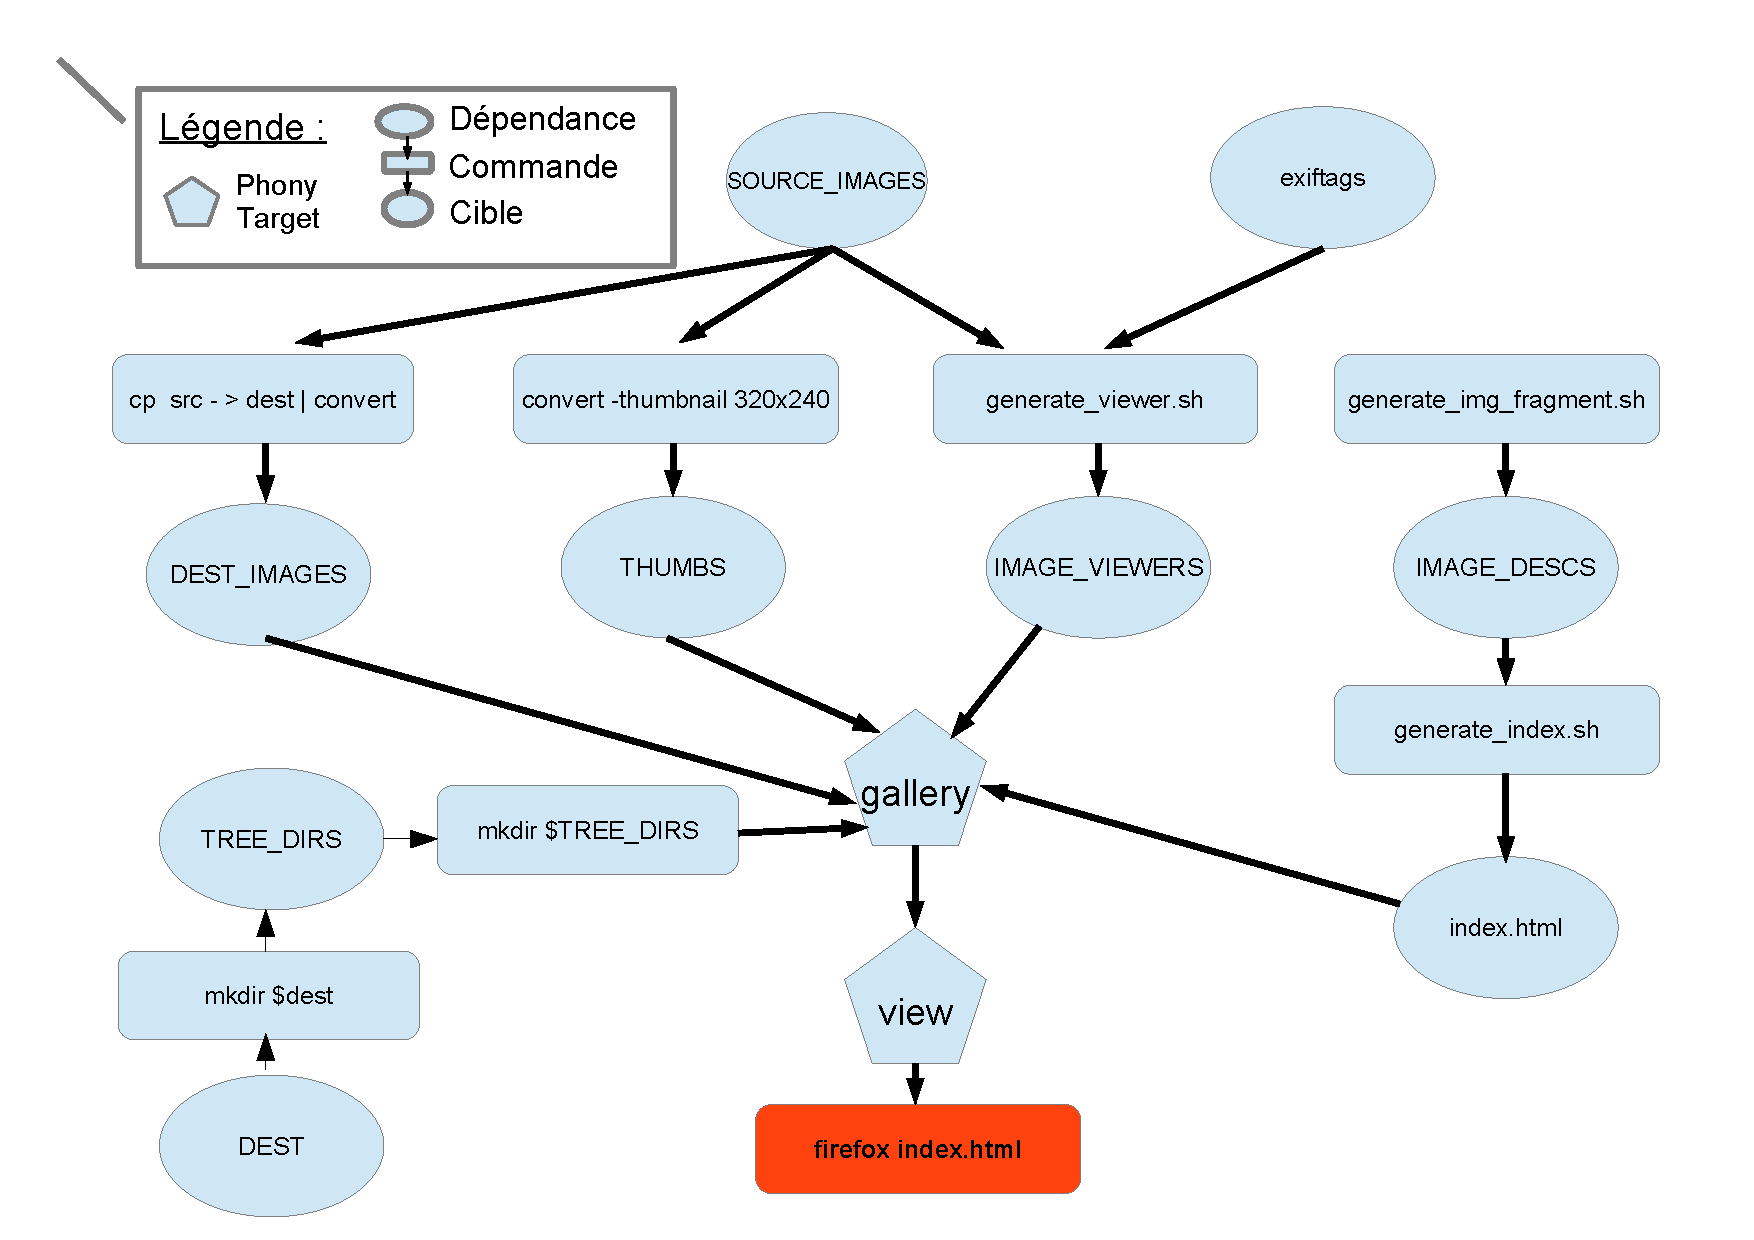
\includegraphics[width=10 cm]{makefile_graph.pdf}
  \caption{Graphe des dépendances et tâches du Makefile}
\end{center}
\label{fig:makefile_graph}
\end{figure}

La Figure ~\ref{fig:makefile_graph} montre de quelle façon est
structuré notre Makefile, par soucis de clarté du schéma, les dépendances entre
\lstinline!TREE\_DIR! et toutes les cibles secondaires, ainsi que les
règles de cleaning et exiftags n'ont pas été représentées.

\begin{figure}[!h]
\begin{center}
  \includegraphics[width=8 cm]{time120-15chart.pdf}
  \caption{Temps d'exécution de make en fonction du degré de
    parallélisme et du nombre d'images}
\end{center}
\label{fig:time_graph}
\end{figure}

Nous avons effectué des mesures de performance de la genération de
gallerie avec divers degrés de parallélisme et 15 ou 100 images, nos
résultats sont observable en Figure ~\ref{fig:time_graph}. 
Quelque soit le nombre d'images, sur la machine ayant effectué les
tests, on obtient un minimum à N = 7 processus en parallèle.

\end{document}
